\section{Bitcoin-NG}
\subsection{介绍}
Bitcoin-NG是另一个针对比特币的扩容限制(scalability limits)提出思考的论文,发表在NSDI16上。其作者之一Ittay Eyal专攻区块链与博弈论相结合的领域,曾提出过selfish mining等著名进攻方式。该论文提出基于比特币的扩展协议旨在满足下面的目标:
\begin{itemize}
	\item Bitcoin-NG的延迟只受限于网络传输的延迟。
	\item Bitcoin-NG的带宽只受限于个人节点的处理容量。
	
\end{itemize}

\subsection{模型}
其主要思想是,允许矿工在挖出一个(主)区块的基础上,按固定速率不断出接在主块之后的子区块(microblocks),直到下一个主区块被挖出。这段时间内这个矿工叫做leader,而只有包含leader有效签名的子区块才会被认可。子区块无需工作量证明,但产出子区块的速率被事先确定。

\begin{figure}
	\centering
	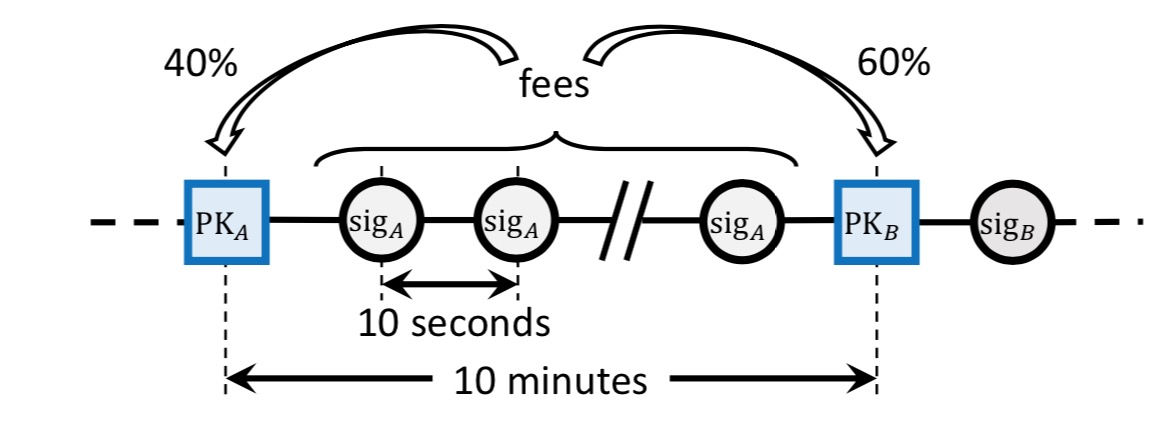
\includegraphics[width=0.7 \textwidth]{../common/BTCNG_1.png}
	\caption{Bitcoint-NG区块结构。其中$40\%$和$60\%$分别为一个子区块的交易费的分配方式,即leader获得$40\%$,挖出下一主块的矿工获得$60\%$} 
	\label{fig:BTCNG1}
\end{figure}
\reffig{fig:BTCNG1}展示了Bitcoin-NG的区块结构以及交易费的分配方式。

值得注意的是,因为每个leader都会尽全力出子区块,所以,当下一个主区块被挖出的时候几乎会必定产生分叉,如图\ref{fig:BTCNG2}。所以,文章指出当用户收到一个子区块的时候,在确认该区块在主链之前应该等一段时间。
\begin{figure}
	\centering
	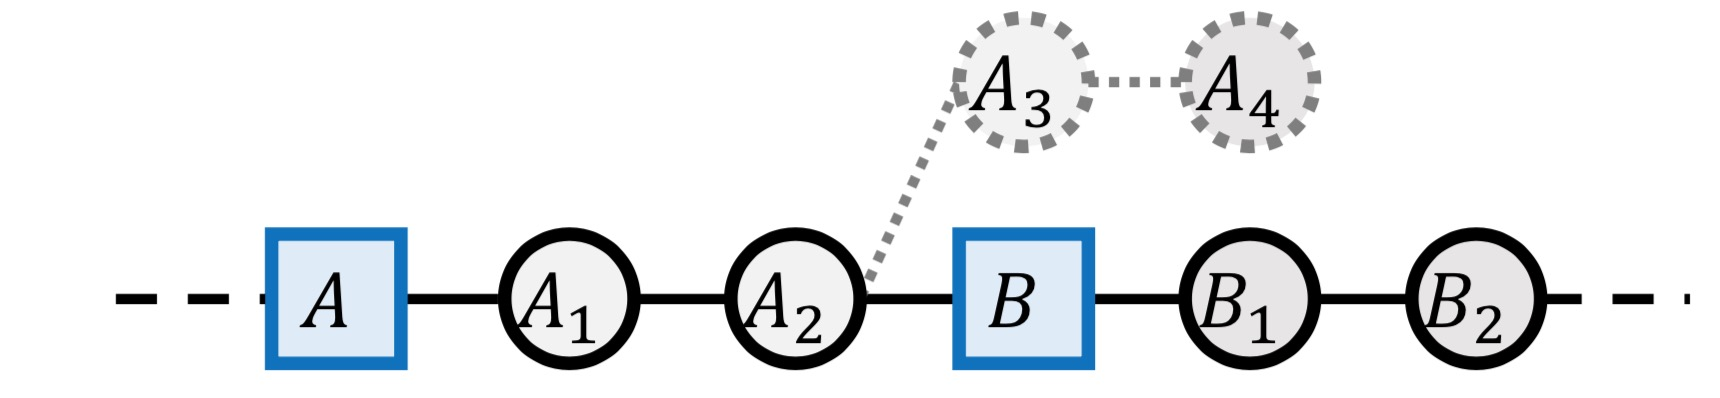
\includegraphics[width=0.7	\textwidth]{../common/BTCNG_2.png}
	\caption{Bitcoint-NG分叉情形:leader $A$一直在出子区块,但是矿工$B$已经在子区块$A_2$后面挖出了一个主块。} 
	\label{fig:BTCNG2}
\end{figure}

同时,因为每个leader拥有自块的任意出块权,他可以选择恶意分叉他出的子区块以实现双花攻击(double spending)。Bitcoin-NG的解决方式是,允许任何用户发送一个有毒交易(poison transaction),这个有毒交易是对分叉行为的一种举报,包含被裁减的分叉的第一个区块的内容,作为“欺骗证明(proof of fraud)”。每个leader需要等待一定的时间(maturity window)才能获得发区块的收益,在这期间内一旦被举报作弊leader将失去收益作为惩罚。同时,发出有毒交易当前leader能获得作弊者赔偿的$5\%$。

\subsection{安全性分析}
Bitcoin-NG假设作恶节点的比例不超过1/4。这是在考虑到了私自挖矿(selfish mining)的情况下。鉴于大量其他共识的论文并没有把私自挖矿考虑进去,这里不做详细介绍。

文章接下来从博弈论角度分析leader的进攻方式。假设每笔交易费有$r_{leader}$(待定)的比例归leader所有,剩下$1-r_{leader}$归挖出下一个区块的矿工所有。假设leader拥有全网$\alpha$比例的算力:
\begin{itemize}
	\item 当leader创建包含某笔交易的子区块时,他不公布这个区块,而是在这个区块之后继续挖矿,期待自己能挖到后继的子区块,这样能获得该笔交易$100\%$的交易费。若失败,该笔交易被部署在其他矿工挖出的子区块上,则该leader回归正常,继续在新的子区块上挖矿。这种行为不会提升该leader的收益当且仅当
	$$ \overbrace{\alpha\times 100\%}^{Win}+\overbrace{(1-\alpha)\times\alpha \times ( 100\%-r_{leader})}^{Lose~but~mine~after~txn}<r_{leader}$$
	当$\alpha<1/4$时,解得$r_{leader} >37\%$
	
	\item 对于某笔交易,leader选择裁减掉这笔交易所在的区块,直接在其之前的区块上挖矿。若leader成功挖出下一个主区块,则他可以将该特定交易部署到自己接下来出的子区块上,并继续挖矿争取能挖到再下一个主区块以获得该笔交易的剩余交易费。相比于直接在这笔交易子区块挖矿,leader的收益不会提升当且仅当
	$$ \overbrace{r_{leader}}^{Place~in~microblock}+\overbrace{ \alpha \times ( 100\%-r_{leader})}^{Lose~but~mine~after~txn} < 100\%-r_{leader}$$
		当$\alpha<1/4$时,解得$r_{leader} < 43\%$
\end{itemize}
故$r_{leader} = 40\%$ 是一个可行的选择。

作为一个博弈论专家,作者接下来考虑的是各种可能的进攻方式以及各类指标(比通常的共识算法考虑的更多)并与比特币进行比较。这里列出一些重点供参考。

1.关于挖矿难度:比特币的挖矿难度是动态调整的,故矿工有动机在难度较高的时候停止挖矿或转向其他公链挖矿,等到难度降低之后再回归。而在Bitcoin-NG中,由于子区块的出块速率是固定的,故只有主区块会受到这种行为的影响。故相对而言影响较小。

2.关于分叉。Bitcoin-NG承认会比比特币拥有更多的分叉,如\reffig{fig:BTCNG2}所示。但是,在Bitcoin-NG中分叉消失的更快,因为一旦一个主区块被挖出则leader权改变,子区块分叉小时。但是对于主区块的分叉并没有解释很清楚。(见原文5.2)

3.文章提出了一些衡量区块链性能的指标,包括共识延迟,公平性,矿力利用率,修剪(分叉被确认忽略)时间,	胜利(主链确认)时间等。文章的实验是基于不同的区块大小和出块评率绘制上述指标的曲线,并与比特币相比较。有兴趣的读者可以参阅原文查看结果。

\subsection{总结}
Bitcoin-NG这种出小块的思想具有一定的借鉴意义,类似于一种锦上添花的功能,但和GHOST一样,对共识原型的贡献不大。同时,文章并没有很显示的证明本章节开头提出的关于比特币扩容的两点。另外,文章提出的各项指标实际被后续工作引用的不多,参考价值有限。

